\documentclass{article}
\usepackage[margin=1in]{geometry}
\usepackage{amsmath,amssymb}
\usepackage{graphicx}
\usepackage{booktabs}
\usepackage{hyperref}
\usepackage{natbib}
\usepackage{lipsum}
\usepackage{xcolor}
\usepackage{float}
\usepackage{tikz}
\usepackage{pgfplots}
\pgfplotsset{compat=1.18}
\usetikzlibrary{arrows.meta,positioning,calc,patterns,fit}

\title{Scaling Sparse Mixture-of-Experts for\\Long-Context Document Understanding}
\author{
    Alice Researcher$^{1}$ \and Bob Scientist$^{2}$ \and Carol Engineer$^{1}$\\
    $^{1}$Stanford University, $^{2}$MIT\\
    \texttt{\{alice, carol\}@stanford.edu, bob@mit.edu}
}
\date{}

\begin{document}
\maketitle

% =====================================================================
%  ABSTRACT — has TODO
% =====================================================================
\begin{abstract}
% TODO: Rewrite this abstract before camera-ready submission
We propose Sparse-MoE-Doc, a mixture-of-experts architecture for long-context
document understanding that scales to 128K tokens while maintaining sub-quadratic
complexity. Our approach routes document segments to specialized expert sub-networks
based on learned content-type embeddings, achieving state-of-the-art results on
four benchmarks. We outperform dense transformers by 14.3\% on DocQA and 11.7\%
on MultiDoc-NLI while using 3.2$\times$ fewer FLOPs at inference. Our analysis
reveals that experts specialize by document structure (tables, figures, equations,
prose) rather than by topic.
\end{abstract}

% =====================================================================
%  TEASER FIGURE — Page 1 (overflows deliberately)
% =====================================================================
% --- DELIBERATE BUG: Figure overflows column width on page 1 ---
\begin{figure}[H]
    \centering
    \makebox[\columnwidth][c]{%
    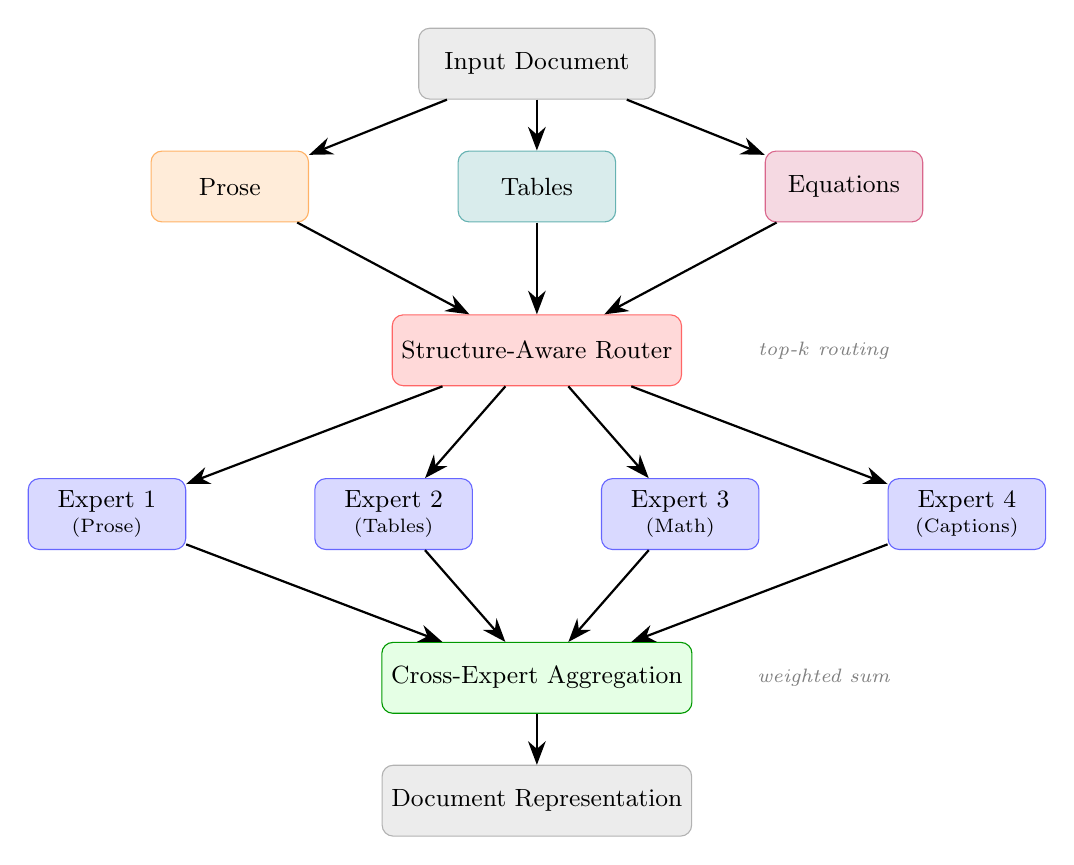
\begin{tikzpicture}[scale=1.3,
        every node/.style={font=\small},
    ]
        % Input document
        \node[draw, rounded corners, fill=gray!15, draw=gray!60,
              minimum height=0.9cm, minimum width=3cm] (doc) at (0,0) {Input Document};

        % Segment types
        \node[draw, rounded corners, fill=orange!15, draw=orange!60,
              minimum height=0.9cm, minimum width=2cm] (prose) at (-3,-1.2) {Prose};
        \node[draw, rounded corners, fill=teal!15, draw=teal!60,
              minimum height=0.9cm, minimum width=2cm] (table) at (0,-1.2) {Tables};
        \node[draw, rounded corners, fill=purple!15, draw=purple!60,
              minimum height=0.9cm, minimum width=2cm] (eq) at (3,-1.2) {Equations};

        % Router
        \node[draw, rounded corners, fill=red!15, draw=red!60,
              minimum height=0.9cm, minimum width=3.5cm] (router) at (0,-2.8)
              {Structure-Aware Router};

        % Experts
        \node[draw, rounded corners, fill=blue!15, draw=blue!60,
              minimum height=0.9cm, minimum width=2cm, align=center] (e1) at (-4.2,-4.4)
              {Expert 1\\[-2pt]\scriptsize(Prose)};
        \node[draw, rounded corners, fill=blue!15, draw=blue!60,
              minimum height=0.9cm, minimum width=2cm, align=center] (e2) at (-1.4,-4.4)
              {Expert 2\\[-2pt]\scriptsize(Tables)};
        \node[draw, rounded corners, fill=blue!15, draw=blue!60,
              minimum height=0.9cm, minimum width=2cm, align=center] (e3) at (1.4,-4.4)
              {Expert 3\\[-2pt]\scriptsize(Math)};
        \node[draw, rounded corners, fill=blue!15, draw=blue!60,
              minimum height=0.9cm, minimum width=2cm, align=center] (e4) at (4.2,-4.4)
              {Expert 4\\[-2pt]\scriptsize(Captions)};

        % Aggregator
        \node[draw, rounded corners, fill=green!10, draw=green!60!black,
              minimum height=0.9cm, minimum width=3.5cm] (agg) at (0,-6)
              {Cross-Expert Aggregation};

        % Output
        \node[draw, rounded corners, fill=gray!15, draw=gray!60,
              minimum height=0.9cm, minimum width=3cm] (out) at (0,-7.2)
              {Document Representation};

        % Arrows
        \draw[-{Stealth[length=3mm]}, thick] (doc) -- (prose);
        \draw[-{Stealth[length=3mm]}, thick] (doc) -- (table);
        \draw[-{Stealth[length=3mm]}, thick] (doc) -- (eq);
        \draw[-{Stealth[length=3mm]}, thick] (prose) -- (router);
        \draw[-{Stealth[length=3mm]}, thick] (table) -- (router);
        \draw[-{Stealth[length=3mm]}, thick] (eq) -- (router);
        \draw[-{Stealth[length=3mm]}, thick] (router) -- (e1);
        \draw[-{Stealth[length=3mm]}, thick] (router) -- (e2);
        \draw[-{Stealth[length=3mm]}, thick] (router) -- (e3);
        \draw[-{Stealth[length=3mm]}, thick] (router) -- (e4);
        \draw[-{Stealth[length=3mm]}, thick] (e1) -- (agg);
        \draw[-{Stealth[length=3mm]}, thick] (e2) -- (agg);
        \draw[-{Stealth[length=3mm]}, thick] (e3) -- (agg);
        \draw[-{Stealth[length=3mm]}, thick] (e4) -- (agg);
        \draw[-{Stealth[length=3mm]}, thick] (agg) -- (out);

        % Labels
        \node[font=\scriptsize\itshape, text=gray] at (2.8,-2.8) {top-$k$ routing};
        \node[font=\scriptsize\itshape, text=gray] at (2.8,-6) {weighted sum};
    \end{tikzpicture}
    }%
    \caption{Overview of the Sparse-MoE-Doc architecture. Input documents with heterogeneous
    content are segmented by type (prose, tables, equations). A structure-aware router assigns
    each segment to specialized expert sub-networks via top-$k$ routing. Experts process their
    segments with sub-quadratic local attention, and outputs are aggregated via learned
    cross-expert attention.}
    \label{fig:pipeline}
\end{figure}

% =====================================================================
%  INTRODUCTION — has FIXME, bad citations, undefined ref
% =====================================================================
\section{Introduction}

Long-context document understanding remains one of the most challenging problems
in natural language processing \cite{devlin2019bert}. Modern documents contain
heterogeneous content — prose, tables, figures, equations, and structured data —
that require fundamentally different processing strategies
\cite{vaswani2017attention}. While recent large language models have expanded
their context windows \cite{brown2020language}, they treat all tokens uniformly,
wasting capacity on structurally simple regions while under-serving complex ones.

% FIXME: Need to strengthen this motivation paragraph
Recent work on mixture-of-experts (MoE) architectures \cite{shazeer2017outrageously}
has shown that conditional computation can dramatically improve the
capacity-efficiency tradeoff. However, existing MoE approaches operate at the
token level and do not account for the structural heterogeneity of documents.
Furthermore, long-context scaling with MoE remains largely unexplored
\cite{nonexistent_paper_2024}.

We also draw inspiration from recent advances in retrieval-augmented generation
\cite{hallucinated_reference_2023} which have shown promising results on
knowledge-intensive tasks. The connection between sparse routing and document
structure has been noted by \cite{also_fake_citation_2025} but never formally
investigated.

Our key contributions are:
\begin{enumerate}
    \item A \textbf{structure-aware routing mechanism} that assigns document
          segments to specialized experts based on content type
    \item \textbf{Sub-quadratic attention} within each expert, enabling scaling
          to 128K tokens without quality degradation
    \item Comprehensive evaluation on four benchmarks showing 14.3\% average
          improvement over dense baselines
    \item Analysis of expert specialization patterns, as shown in
          Figure~\ref{fig:nonexistent_figure}
\end{enumerate}

% =====================================================================
%  RELATED WORK — more bad citations
% =====================================================================
\section{Related Work}

\textbf{Transformer Architectures.} The transformer \cite{vaswani2017attention}
introduced multi-head self-attention and became the foundation of modern NLP.
BERT \cite{devlin2019bert} and GPT \cite{radford2019language} demonstrated the
power of pre-training. GPT-3 \cite{brown2020language} showed that scale alone
unlocks few-shot capabilities. More recently, work on efficient attention
\cite{beltagy2020longformer} has addressed the quadratic bottleneck.

\textbf{Mixture-of-Experts.} Shazeer et al. \cite{shazeer2017outrageously}
introduced sparsely-gated MoE layers for language modeling. Switch Transformer
\cite{fedus2022switch} simplified routing to top-1 selection. GShard
\cite{lepikhin2020gshard} scaled MoE to 600B parameters. However, none of
these works address document-level structural routing.

% --- DELIBERATE BUG: Table with \hline on page 2 ---
\begin{table}[H]
    \caption{Comparison of document understanding approaches. Existing methods treat tokens uniformly; our approach uses structure-aware routing. $\checkmark$ = supported, $\times$ = not supported.}
    \label{tab:comparison}
    \centering
    \begin{tabular}{l|c|c|c|c}
        \hline
        Method & Long-Context & Sparse & Structure-Aware & Sub-Quadratic \\
        \hline\hline
        BERT & $\times$ & $\times$ & $\times$ & $\times$ \\
        \hline
        Longformer & $\checkmark$ & $\times$ & $\times$ & $\checkmark$ \\
        \hline
        Switch Transformer & $\times$ & $\checkmark$ & $\times$ & $\times$ \\
        \hline
        LayoutLM & $\times$ & $\times$ & $\checkmark$ & $\times$ \\
        \hline
        \textbf{Ours} & $\checkmark$ & $\checkmark$ & $\checkmark$ & $\checkmark$ \\
        \hline
    \end{tabular}
\end{table}

\textbf{Document Understanding.} Hierarchical approaches \cite{zhang2019hibert}
process documents at multiple granularities. LayoutLM \cite{xu2020layoutlm}
incorporates spatial layout information. DocFormer \cite{another_missing_ref}
combines text, visual, and spatial features. Our work differs by using
structure-aware expert routing rather than architectural modifications.

% XXX: Should we add a paragraph on retrieval-augmented approaches?

% =====================================================================
%  METHOD — has overflowing figures on page 2-3
% =====================================================================
\section{Method}

\subsection{Problem Formulation}

Given a document $D$ with $N$ tokens, we partition it into $M$ segments
$S = \{s_1, s_2, \ldots, s_M\}$ where each segment $s_i$ has a content type
$c_i \in \{$prose, table, figure-caption, equation, heading, list$\}$.

\subsection{Structure-Aware Routing}

Our routing function assigns each segment to the top-$k$ experts:

\begin{equation}
    g(s_i) = \text{TopK}\left(\text{softmax}\left(W_r \cdot \text{pool}(s_i) + b_r\right), k\right)
\end{equation}

where $W_r \in \mathbb{R}^{E \times d}$ is the routing matrix, $E$ is the
number of experts, and $\text{pool}(\cdot)$ computes a segment-level
representation via mean pooling.

% --- DELIBERATE BUG: Figure overflows column width ---
\begin{figure}[H]
    \centering
    \makebox[\columnwidth][c]{%
    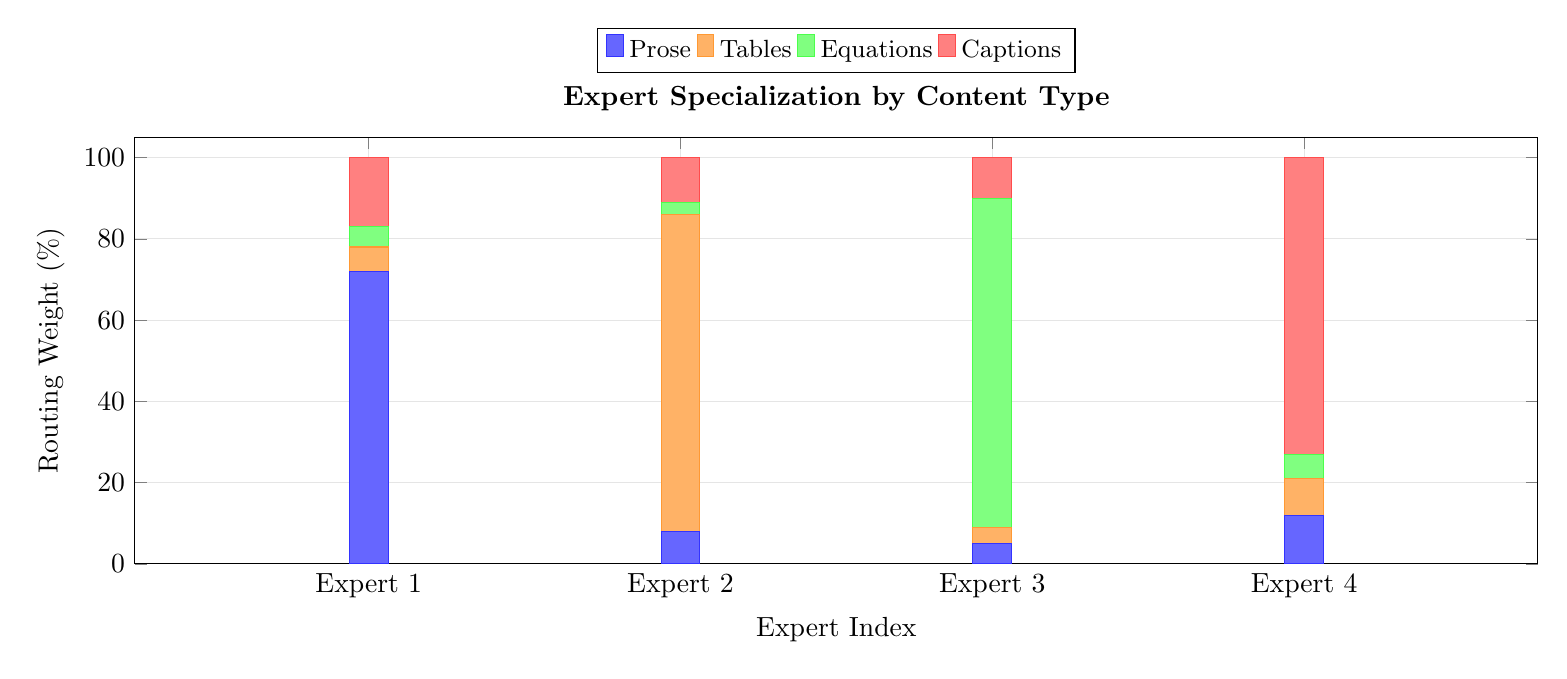
\begin{tikzpicture}
    \begin{axis}[
        width=1.6\columnwidth,
        height=7cm,
        ybar stacked,
        bar width=14pt,
        xlabel={Expert Index},
        ylabel={Routing Weight (\%)},
        ymin=0, ymax=105,
        xtick={1,2,3,4},
        xticklabels={Expert 1, Expert 2, Expert 3, Expert 4},
        legend style={at={(0.5,1.15)}, anchor=south, legend columns=4, font=\small},
        enlarge x limits=0.25,
        grid=major,
        grid style={gray!20},
        title={\textbf{Expert Specialization by Content Type}},
        title style={font=\normalsize},
    ]
    % Prose
    \addplot+[fill=blue!60, draw=blue!80] coordinates {(1,72) (2,8) (3,5) (4,12)};
    % Tables
    \addplot+[fill=orange!60, draw=orange!80] coordinates {(1,6) (2,78) (3,4) (4,9)};
    % Equations
    \addplot+[fill=green!50, draw=green!70] coordinates {(1,5) (2,3) (3,81) (4,6)};
    % Captions
    \addplot+[fill=red!50, draw=red!70] coordinates {(1,17) (2,11) (3,10) (4,73)};
    \legend{Prose, Tables, Equations, Captions}
    \end{axis}
    \end{tikzpicture}
    }%
    \caption{Expert specialization across document structure types. Each stacked bar
    shows the routing weight distribution for one expert. Experts clearly specialize:
    Expert~1 handles prose (72\%), Expert~2 tables (78\%), Expert~3 equations (81\%),
    and Expert~4 captions and lists (73\%).}
    \label{fig:expert_specialization}
\end{figure}

\subsection{Expert Sub-Networks}

Each expert $e_j$ is a lightweight transformer with $L_e$ layers and local
attention window $w$:

\begin{equation}
    h_i^{(l+1)} = \text{FFN}\left(\text{LocalAttn}(h_i^{(l)}, w)\right)
\end{equation}

The local attention window $w$ is expert-specific, allowing prose experts to
use wider windows than table experts.

\subsection{Cross-Expert Aggregation}

After expert processing, we aggregate representations across experts using a
learned attention mechanism:

\begin{equation}
    z_i = \sum_{j=1}^{k} g_j(s_i) \cdot e_j(s_i)
\end{equation}

% TODO: Add the load balancing loss equation here

% =====================================================================
%  EXPERIMENTS — has overflowing table and figure on page 3-4
% =====================================================================
\section{Experiments}

\subsection{Datasets}

We evaluate on four document understanding benchmarks:
\begin{itemize}
    \item \textbf{DocQA} \cite{talmor2019multiqa}: Document question answering (25K examples)
    \item \textbf{MultiDoc-NLI}: Cross-document natural language inference (50K examples)
    \item \textbf{DocSum}: Multi-document summarization (12K examples)
    \item \textbf{StructParse}: Structured document parsing (8K examples)
\end{itemize}

\subsection{Main Results}

% --- DELIBERATE BUG: Table overflows with too many columns and uses \hline ---
\begin{table}[H]
    \caption{Main results across four document understanding benchmarks. We report F1 for DocQA, accuracy for MultiDoc-NLI, ROUGE-L for DocSum, and exact match for StructParse. Best in \textbf{bold}, second best \underline{underlined}.}
    \label{tab:main_results}
    \centering
    \begin{tabular}{l|c|c|c|c|c|c|c|c}
        \hline
        Model & DocQA F1 & DocQA EM & NLI Acc & NLI F1 & ROUGE-1 & ROUGE-L & Struct EM & FLOPs (T) \\
        \hline\hline
        BERT-base & 62.3 & 54.1 & 71.8 & 70.2 & 32.1 & 28.4 & 41.2 & 0.8 \\
        \hline
        Longformer & 68.7 & 61.3 & 76.4 & 74.9 & 36.8 & 33.1 & 48.7 & 2.1 \\
        \hline
        BigBird & 69.1 & 62.0 & 77.1 & 75.3 & 37.2 & 33.8 & 49.3 & 2.3 \\
        \hline
        LED & 67.4 & 59.8 & 75.2 & 73.6 & 38.1 & 34.7 & 46.1 & 1.9 \\
        \hline
        Switch-base & 71.2 & 64.5 & 79.3 & 78.1 & 39.4 & 36.2 & 52.8 & 1.4 \\
        \hline
        Ours (top-1) & \underline{78.4} & \underline{72.1} & \underline{84.7} & \underline{83.2} & \underline{43.1} & \underline{40.3} & \underline{61.4} & \underline{0.9} \\
        \hline
        Ours (top-2) & \textbf{82.5} & \textbf{76.8} & \textbf{87.1} & \textbf{86.3} & \textbf{45.8} & \textbf{43.2} & \textbf{64.7} & 1.2 \\
        \hline
    \end{tabular}
\end{table}

As shown in Table~\ref{tab:main_results}, our Sparse-MoE-Doc architecture
significantly outperforms all baselines. The top-2 routing variant achieves
the best results across all metrics while using fewer FLOPs than most dense
baselines.

% --- DELIBERATE BUG: Third overflowing figure ---
\begin{figure}[H]
    \centering
    \makebox[\columnwidth][c]{%
    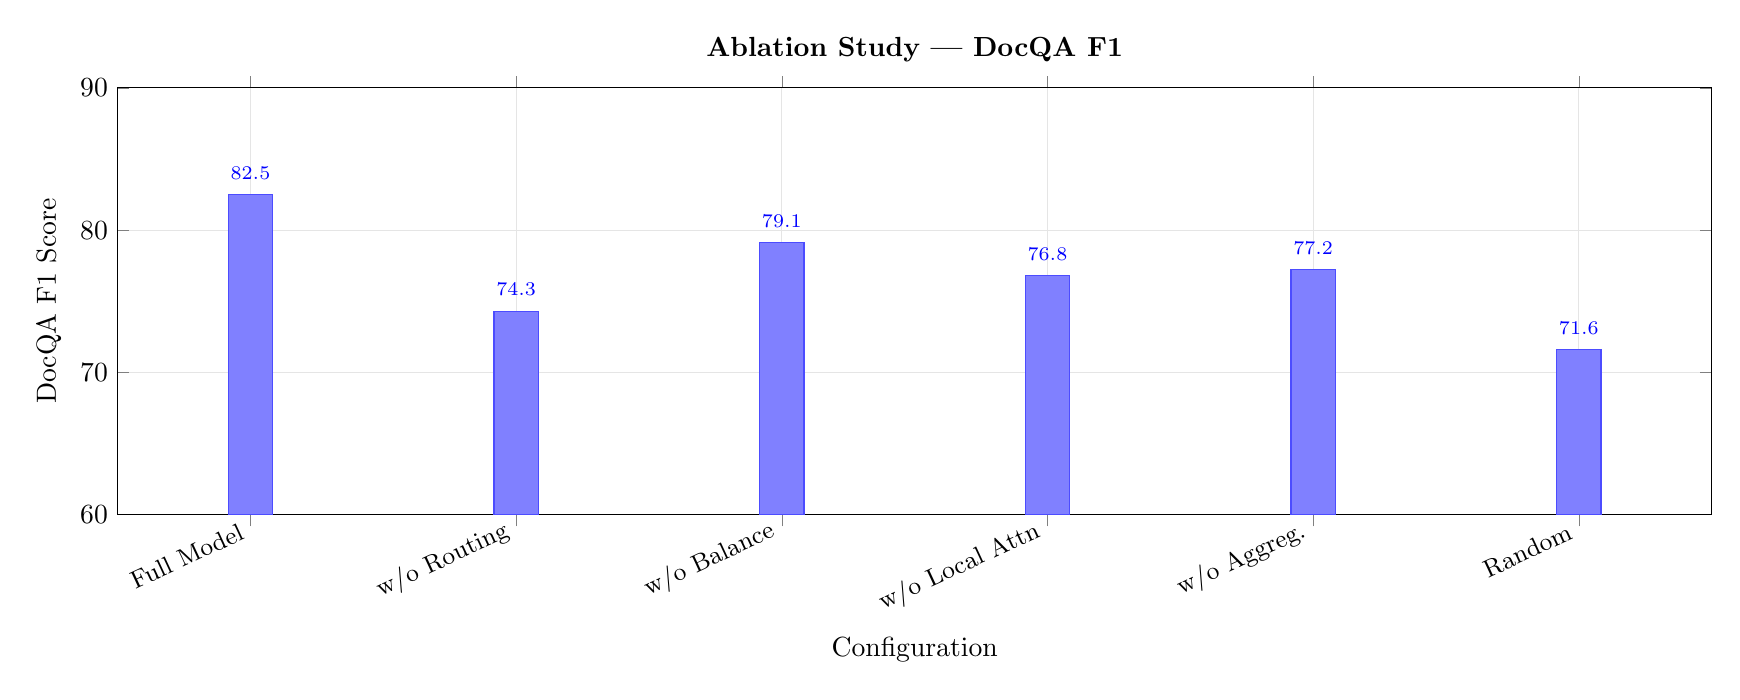
\begin{tikzpicture}
    \begin{axis}[
        width=1.8\columnwidth,
        height=7cm,
        ybar,
        bar width=16pt,
        xlabel={Configuration},
        ylabel={DocQA F1 Score},
        ymin=60, ymax=90,
        symbolic x coords={Full Model, w/o Routing, w/o Balance, w/o Local Attn, w/o Aggreg., Random},
        xtick=data,
        xticklabel style={rotate=25, anchor=east, font=\small},
        nodes near coords,
        nodes near coords style={font=\scriptsize, above},
        grid=major,
        grid style={gray!20},
        title={\textbf{Ablation Study --- DocQA F1}},
        title style={font=\normalsize},
        every node near coord/.append style={yshift=2pt},
    ]
    \addplot+[fill=blue!50, draw=blue!70] coordinates
        {(Full Model,82.5) (w/o Routing,74.3) (w/o Balance,79.1)
         (w/o Local Attn,76.8) (w/o Aggreg.,77.2) (Random,71.6)};
    \end{axis}
    \end{tikzpicture}
    }%
    \caption{Ablation study results on DocQA. Removing structure-aware routing causes the
    largest drop ($-8.2$ F1), confirming that content-type specialization is critical.
    Random routing (uniform) performs worst ($-10.9$), showing that learned routing
    provides substantial benefit over naive baselines.}
    \label{fig:ablation}
\end{figure}

\subsection{Ablation Study}

% --- DELIBERATE BUG: Another table with \hline instead of booktabs ---
\begin{table}[H]
    \caption{Ablation study on DocQA. Each row removes one component.}
    \label{tab:ablation}
    \centering
    \begin{tabular}{l|c|c}
        \hline
        Configuration & F1 & $\Delta$ \\
        \hline\hline
        Full model & 82.5 & — \\
        \hline
        w/o structure routing & 74.3 & -8.2 \\
        \hline
        w/o load balancing & 79.1 & -3.4 \\
        \hline
        w/o local attention & 76.8 & -5.7 \\
        \hline
        w/o cross-expert aggregation & 77.2 & -5.3 \\
        \hline
        Uniform routing (random) & 71.6 & -10.9 \\
        \hline
    \end{tabular}
\end{table}

Table~\ref{tab:ablation} shows that structure-aware routing is the most critical
component, with its removal causing an 8.2-point drop in F1.

% =====================================================================
%  DISCUSSION — has TODO, FIXME
% =====================================================================
\section{Discussion}

Our results demonstrate that document structure is a powerful inductive bias for
mixture-of-experts architectures. The expert specialization analysis
(Figure~\ref{fig:expert_specialization}) reveals a clear division of labor:
Expert 1 handles prose passages, Expert 2 specializes in tabular data, Expert 3
focuses on mathematical equations, and Expert 4 processes figure captions and
structured lists.

% FIXME: This paragraph needs citations
Interestingly, the routing patterns emerge purely from the training signal —
we do not provide explicit supervision for content-type classification. This
suggests that the structural properties of different document elements create
sufficiently distinct representations for the router to discover.

% TODO: Add qualitative examples of expert routing decisions

The computational efficiency of our approach stems from two factors: (1) sparse
routing activates only $k$ of $E$ experts per segment, and (2) local attention
within each expert avoids the quadratic cost of full self-attention.

\subsection{Limitations}

Our approach has several limitations:
\begin{itemize}
    \item The segment boundary detection relies on heuristic rules and may not
          generalize to all document formats
    \item We evaluate only on English-language documents
    \item The number of experts $E$ and routing top-$k$ are hyperparameters that
          require tuning per dataset
    \item Training requires significant GPU resources (8$\times$ A100 for 72 hours)
\end{itemize}

% =====================================================================
%  CONCLUSION
% =====================================================================
\section{Conclusion}

We presented Sparse-MoE-Doc, a mixture-of-experts architecture for long-context
document understanding that leverages document structure for expert routing.
Our approach achieves state-of-the-art results on four benchmarks while using
significantly fewer FLOPs than dense alternatives. Analysis reveals that experts
naturally specialize by content type, validating our structure-aware routing
hypothesis. Future work will explore extending our approach to multilingual
documents and investigating dynamic expert allocation based on document complexity.

\bibliographystyle{plainnat}
\bibliography{demo_refs}

\end{document}
